\documentclass[degree=master]{thuthesis}
% 选项:
%   degree=[bachelor|master|doctor|postdoctor], % 必选
%   secret,                                     % 可选
%   pifootnote,                                 % 可选(建议打开)
%   openany|openright,                          % 可选,基本不用
%   arial,                                      % 可选,基本不用
%   arialtoc,                                   % 可选,基本不用
%   arialtitle                                  % 可选,基本不用

% 所有其它可能用到的包都统一放到这里了,可以根据自己的实际添加或者删除。
\usepackage{thuthesis}

% 定义所有的图片文件在 figures 子目录下
\graphicspath{{figures/}}

% 可以在这里修改配置文件中的定义。导言区可以使用中文。
% \def\myname{薛瑞尼}

\begin{document}

%%% 封面部分
\frontmatter
\thusetup{
  %******************************
  % 注意:
  %   1. 配置里面不要出现空行
  %   2. 不需要的配置信息可以删除
  %******************************
  %
  %=====
  % 秘级
  %=====
  secretlevel={秘密},
  secretyear={10},
  %
  %=========
  % 中文信息
  %=========
  ctitle={清华大学学位论文 \LaTeX\ 模板\\使用示例文档 v\version},
  cdegree={工程硕士},
  cdepartment={计算机科学与技术系},
  cmajor={计算机技术},
  cauthor={朱洁},
  csupervisor={李琦副研究员},
  %cassosupervisor={陈文光教授}, % 副指导老师
  %ccosupervisor={王聪教授,王骞教授}, % 联合指导老师
  % 日期自动使用当前时间,若需指定按如下方式修改:
  % cdate={超新星纪元},
  %
  % 博士后专有部分
  cfirstdiscipline={计算机科学与技术},
  cseconddiscipline={系统结构},
  postdoctordate={2009年7月——2011年7月},
  id={编号}, % 可以留空: id={},
  udc={UDC}, % 可以留空
  catalognumber={分类号}, % 可以留空
  %
  %=========
  % 英文信息
  %=========
  etitle={An Introduction to \LaTeX{} Thesis Template of Tsinghua University v\version},
  % 这块比较复杂,需要分情况讨论:
  % 1. 学术型硕士
  %    edegree:必须为Master of Arts或Master of Science(注意大小写)
  %             “哲学、文学、历史学、法学、教育学、艺术学门类,公共管理学科
  %              填写Master of Arts,其它填写Master of Science”
  %    emajor:“获得一级学科授权的学科填写一级学科名称,其它填写二级学科名称”
  % 2. 专业型硕士
  %    edegree:“填写专业学位英文名称全称”
  %    emajor:“工程硕士填写工程领域,其它专业学位不填写此项”
  % 3. 学术型博士
  %    edegree:Doctor of Philosophy(注意大小写)
  %    emajor:“获得一级学科授权的学科填写一级学科名称,其它填写二级学科名称”
  % 4. 专业型博士
  %    edegree:“填写专业学位英文名称全称”
  %    emajor:不填写此项
  edegree={Master of Engineering},
  emajor={Computer Science and Technology},
  eauthor={Zhu Jie},
  esupervisor={Professor Li Qi},
  %eassosupervisor={Chen Wenguang},
  % 日期自动生成,若需指定按如下方式修改:
  % edate={December, 2005}
  %
  % 关键词用“英文逗号”分割
  ckeywords={\TeX, \LaTeX, CJK, 模板, 论文},
  ekeywords={\TeX, \LaTeX, CJK, template, thesis}
}

% 定义中英文摘要和关键字
\begin{cabstract}
  论文的摘要是对论文研究内容和成果的高度概括。摘要应对论文所研究的问题及其研究目
  的进行描述,对研究方法和过程进行简单介绍,对研究成果和所得结论进行概括。摘要应
  具有独立性和自明性,其内容应包含与论文全文同等量的主要信息。使读者即使不阅读全
  文,通过摘要就能了解论文的总体内容和主要成果。

  论文摘要的书写应力求精确、简明。切忌写成对论文书写内容进行提要的形式,尤其要避
  免“第 1 章……;第 2 章……;……”这种或类似的陈述方式。

  本文介绍清华大学论文模板 \thuthesis{} 的使用方法。本模板符合学校的本科、硕士、
  博士论文格式要求。

  本文的创新点主要有:
  \begin{itemize}
    \item 用例子来解释模板的使用方法;
    \item 用废话来填充无关紧要的部分;
    \item 一边学习摸索一边编写新代码。
  \end{itemize}

  关键词是为了文献标引工作、用以表示全文主要内容信息的单词或术语。关键词不超过 5
  个,每个关键词中间用分号分隔。(模板作者注:关键词分隔符不用考虑,模板会自动处
  理。英文关键词同理。)
\end{cabstract}

% 如果习惯关键字跟在摘要文字后面,可以用直接命令来设置,如下:
% \ckeywords{\TeX, \LaTeX, CJK, 模板, 论文}

\begin{eabstract}
   An abstract of a dissertation is a summary and extraction of research work
   and contributions. Included in an abstract should be description of research
   topic and research objective, brief introduction to methodology and research
   process, and summarization of conclusion and contributions of the
   research. An abstract should be characterized by independence and clarity and
   carry identical information with the dissertation. It should be such that the
   general idea and major contributions of the dissertation are conveyed without
   reading the dissertation.

   An abstract should be concise and to the point. It is a misunderstanding to
   make an abstract an outline of the dissertation and words ``the first
   chapter'', ``the second chapter'' and the like should be avoided in the
   abstract.

   Key words are terms used in a dissertation for indexing, reflecting core
   information of the dissertation. An abstract may contain a maximum of 5 key
   words, with semi-colons used in between to separate one another.
\end{eabstract}

% \ekeywords{\TeX, \LaTeX, CJK, template, thesis}

% 如果使用授权说明扫描页,将可选参数中指定为扫描得到的 PDF 文件名,例如:
% \makecover[scan-auth.pdf]
\makecover

%% 目录
\tableofcontents

%% 符号对照表
\begin{denotation}[3cm]
\item[SSE] 加密搜索 (Searchable Symmetric Encryption)
\item[VSSE] 可验证加密搜索 (Verifiable Searchable Symmetric Encryption)
\item[MPT] 默克尔帕特里夏树 (Merkle Patricia Tree)
\item[IH] 增量哈希 (Incremental Hash)
\item[$\mathcal{W}$] 关键字集合
\item[$|W|$] 关键字集合大小
\item[$w_i$ ] 关键字,其中$i \in \{1, \cdots, |W|\}$
\item[$\mathcal{D}$] 明文文件集合
\item[$D_{w_i}$] 包含关键字$w_i$的明文文件集合
\item[$\mathcal{C}$] 密文文件集合
\item[$C_{w_i}$] 包含关键字$w_i$的密文文件集合
\item[$d$] 明文文件
\item[$c$] 密文文件
\item[$W_d$] 文件$d$包含的关键字集合
\item[$\tau$]	搜索令牌
\item[$\lambda$] 验证索引
\item[$\pi$] 鉴别符
\end{denotation}



%%% 正文部分
\mainmatter
\chapter{绪论}
\label{cha:intro}
\section{研究背景及选题意义}
随着云计算技术的发展与日渐成熟,云存储技术也被广泛提及。对个人用户来说,云存储技术通过提高存储效率,为其节省了大量本地存储空间,也便于用户随时随地存储数据,同时云存储技术还为多人之间的数据共享提供了高效的解决方案。对于企业用户来说,云存储技术通过虚拟化技术进行了资源整合,提高了存储空间的利用率,同时云存储技术具备的负载均衡、故障冗余等功能也确保了企业级数据的安全。目前,云存储技术主要分为私有云、公有云和混合云三个类别。其中私有云存储技术主要面向企业用户,为其提供一个安全、高效的云存储环境。一般来说,私有云往往部署在企业内部的数据中心内,它将数据维护在企业防火墙之内,因此安全性较高。而公有云存储业务则向互联网开放,其计算资源相对私有云有很大的优势,但其安全性相对私有云大大降低。公有云存储业务主要面向个人消费者,目前几乎任何一家大型互联网公司都在为用户提供公有云存储服务,例如,Google Drive,iCloud,Dropbox,百度云等等。但公有云存储确实导致了许多安全性问题的产生,例如,数据丢失,数据隐私泄露等等。iCloud曾在2014年出现过严重的数据泄露事件,导致用户对其信任度大大降低,Dropbox也出现过类似事件。总体来说,云存储技术虽然使得用户可以随时随地地存取数据,方便了用户之间的数据共享,降低了维护数据的成本~\cite{juels2007pors,ateniese2008scalable,kamara2011cs2,wang2011enabling,stefanov2012iris,kamara2013parallel,sun2015catch},但其带来的安全问题也不容忽视。云存储带来的安全性问题可以分为以下两类:
\begin{itemize}
	\item 可用性问题。要求云服务器保证数据不丢失,用户可以将云服务器作为数据中枢进行数据备份和同步。目前,一般的云服务提供商都采用了多副本的方式来保障数据的可用性,即将数据的多个副本分别写入其他的存储节点,当一个节点发生故障时,其他节点继续提供服务,同时通过其他节点中的数据副本,快速恢复故障节点上丢失的数据。目前,针对数据可用性的相关学术研究包括数据拥有证明 (Proof of Data Possession, PDP)~\cite{ateniese2007provable, ateniese2008scalable,curtmola2008mr, erway2015dynamic,zhu2012cooperative} ,数据可恢复性证明 (Proof of Retrievability, PoR)~\cite{juels2007pors, bowers2009proofs, stefanov2012iris},数据审计 (Data Auditing)~\cite{wang2010privacy,wang2010toward,wang2013privacy,wang2011enabling,zhu2011dynamic}等等;
	\item 隐私性问题。要求云服务器保证数据的隐私并且不泄露数据。目前,云服务提供商一般采用数据加密方式对隐私数据进行保护,但数据加密往往会导致数据可用性的降低,例如数据失去可搜索性。因此加密搜索 (Searchable Encryption, SE) 随之产生。加密搜索方案按照采用的秘钥机制不同可以分为两类,一是对称加密搜索 (Searchable Symmetric Encryption, SSE)\cite{song2000practical,curtmola2011searchable,kamara2012dynamic,cash2014dynamic,wang2016searchable},二是公钥加密搜索 (Public Key Encryption with Keyword Search, PEKS)~\cite{boneh2004public}。
\end{itemize}

加密搜索的提出,使得用户可以在上传数据给云服务器之前,对其进行加密,并且使得云服务器可以在加密数据上进行搜索。从而既保证了数据的隐私性,又保证了数据的可搜索性。目前,由于效率问题,应用较为广泛的为对称加密搜索技术。然而,大部分的对称加密搜索方案都基于服务器是半可信的假设~\cite{curtmola2011searchable, kamara2012dynamic, cash2014dynamic},即服务器会遵循协议但是可以从用户的查询中推断相关信息。这种假设在实际应用场景中往往是不成立的。因为云服务器可能会因为外部攻击,内部配置错误,软件错误等等问题而导致其违反原有协议~\cite{sun2015catch,bost2016verifiable}。这种协议违反所导致的最常见问题就是服务器返回的搜索结果不完整。例如,云服务器有可能为了节省计算开销和通信开销而返回少量搜索结果给用户,甚至有可能不返回搜索结果给用户。


为了解决该问题,可验证对称加密搜索 (Verifiable Searchable Symmetric Encryption, VSSE) 技术也相应提出\cite{kamara2011cs2,kurosawa2012uc,chai2012verifiable,kurosawa2013update,stefanov2014practical,cheng2015verifiable,bost2016verifiable,ogataefficient}。可验证对称加密搜索技术允许用户对搜索结果进行验证,从而来检测云服务器的不诚信行为,保障加密搜索的正确性。然而,据我们所知,现有的可验证对称加密搜索方案都是不完善的。例如,有的方案~\cite{kurosawa2012uc,chai2012verifiable,cheng2015verifiable,ogataefficient}不支持数据更新,只能作用在静态数据库中,数据库若有变化则需要重建整个索引。有的方案~\cite{kamara2011cs2,kurosawa2013update,stefanov2014practical}无法防止服务器故意返回空结果来规避结果验证。即,这些方案\cite{kamara2011cs2,kurosawa2013update,stefanov2014practical}在用户提交的关键字不存在于数据库中时,是不返回任何搜索结果的。这就导致了服务器可以对任意关键字返回空结果来规避结果验证,除非用户在本地保留数据库的所有关键字集合。另外,大部分的可验证对称加密搜索方案~\cite{kamara2011cs2,kurosawa2012uc,chai2012verifiable,kurosawa2013update,stefanov2014practical,
cheng2015verifiable,ogataefficient,bost2016verifiable}仅仅支持在单用户场景下工作,即数据持有者自己写自己读的场景,而现实情况中,数据往往有共享需求,即一方写多方读的多用户场景\footnote{本文所述的多用户场景指一方写入,多方读取的场景,下文中若不做特别说明,均指这种情况。}。表格~\ref{tab:comparison}比较了现有可验证对称加密搜索方案的功能。



\begin{table}[t]
  \begin{center}
  \caption{现有可验证对称加密搜索方案比较}
  \label{tab:comparison}
  %\begin{threeparttable}
  \begin{tabular}{c c c c c c c}
    \toprule[1.5pt]
                                          &动态$^1$         &新鲜性$^2$     &完整性$^3$    &验证效率$^4$        &通用$^5$  &多用户 \\
    \midrule[1pt]
    KPR11~\cite{kamara2011cs2}            &\checkmark          &\checkmark         &\texttimes                          &$O(|W|)$                      &\checkmark  &\texttimes\\

    KO12~\cite{kurosawa2012uc}            &\texttimes          &\text{-}           &\texttimes                          &$O(n)$                        &\texttimes	&\texttimes\\

    CG12~\cite{chai2012verifiable}        &\texttimes          &\text{-}           &\checkmark                          &$O(log(|W|))$                 &\texttimes  &\texttimes\\

    KO13~\cite{kurosawa2013update}        &\checkmark          &\checkmark         &\texttimes                          &$O(n)$                        &\texttimes 	&\texttimes\\

    SPS14~\cite{stefanov2014practical}    &\checkmark         &\checkmark         &\texttimes                          &$min\{\alpha+log(N), r log^3(N)\}$    &\texttimes &\texttimes\\

    CYG15\cite{cheng2015verifiable}    &\texttimes           &\text{-}         &\texttimes                            &$O(|W|)+O(r)$                 &\texttimes &\texttimes\\

    BFP16~\cite{bost2016verifiable}       &\checkmark          &\checkmark         &\checkmark                          &$O(r)$                        &\checkmark   &\texttimes\\

    OK16~\cite{ogataefficient}            &\texttimes          &\text{-}           &\checkmark                          &$O(r)$                        &\checkmark  &\texttimes\\

    \bottomrule[1.5pt]
  \end{tabular}\\
  \end{center}
	$^1$ \wuhao{注意,动态是指方案是否支持用户数据动态更新,由此可将可验证对称加密搜索方案分为静态和动态两种类型,后者在功能性上更完善。}\\
  $^2$ \wuhao{注意,'\texttimes' 表示有实现的需求但是该方案没有实现, 而 '-' 表示没有实现的需求。具体而言,静态的可验证对称加密搜索方案不存在数据新鲜性问题,因此方案~\cite{kurosawa2012uc,chai2012verifiable,cheng2015verifiable,ogataefficient}也没有进行数据新鲜性验证的需求。}\\
  $^3$ \wuhao{我们考虑各种数据完整性攻击,尤其包括服务器故意返回空结果来规避结果验证的场景。}\\
  $^4$ \wuhao{验证效率是指服务器进行结果验证支持所需要的计算开销。对于表格中的非通用型方案~\cite{kurosawa2012uc,chai2012verifiable,kurosawa2013update,stefanov2014practical,cheng2015verifiable}来说,由于他们的方案并没有将验证索引从加密搜索方案中解耦,因此他们的验证效率和服务器进行加密搜索所需的计算开销是等价的。这里,$n$ 代表所有文件的数量, $|W|$ 表示所有关键字的数量, $r$ 表示包含某一特定关键字的文件数量, $\alpha$ 表示某一关键字历史上被加入到集合中的次数~\cite{stefanov2014practical}, $N$ 表示键值对 (文件,关键字) 对的数量。}\\
  $^5$ \wuhao{一个通用的可验证对称加密搜索方案是指该方案可以为任何加密搜索方案提供结果验证的功能,而非通用的可验证对称加密搜索方案表示该方案仅支持在特定的加密搜索方案下工作。}\\
\end{table}

\section{研究现状}
\subsection{安全云存储方案}
可验证的云存储服务已经被广泛的研究过,例如,数据拥有性证明~\cite{ateniese2007provable, ateniese2008scalable,curtmola2008mr, erway2015dynamic,zhu2012cooperative},数据可取回证明~\cite{juels2007pors, bowers2009proofs, stefanov2012iris},数据审计~\cite{wang2010privacy,wang2010toward,wang2013privacy,wang2011enabling,zhu2011dynamic}等等。这些方案主要侧重于云端存储数据的完整性验证,并支持丢失数据的恢复。注意,这些方案与加密搜索场景下的结果验证是不同的。因为加密搜索的结果验证不仅需要验证某个文件本身的完整性,还需要验证整个搜索结果集合是否完整。而这些方案只能单纯验证数据块的完整性,不支持对搜索结果完整性的验证。

\subsection{安全加密搜索方案}
加密搜索的概念首次由Song等人~\cite{song2000practical}在2000年提出,他们的方案允许用户将加密后的数据集存储到云端,并同时保证用户在该加密数据集上进行搜索的能力。随后,加密搜索方案被广泛的研究,总体来说可以分为以下两个分支:对称加密搜索 (Searchable Symmetric Encryption, SSE)和公钥加密搜索 (Public Key Encryption with Keyword Search, PEKS)。其中,最经典的对称加密搜索方案~\cite{curtmola2011searchable}由Curtmola等人提出,他们对加密搜索的安全性进行了严格的定义,提出加密搜索方案至少要在面对一个被动敌手(Passive Adversary)的情况下是安全可靠的。他们的方案利用了明文搜索中的倒排索引 (Inverted Index) 思想,在效率和安全性上较已有的方案都有较大提升。目前还有许多不同的对称加密搜索方案实现了不同的搜索功能。例如,动态对称加密搜索 (Dynamic SSE) 方案~\cite{kamara2012dynamic,cash2014dynamic,stefanov2014practical}允许用户更新其数据集, 支持关键字排序 (Ranked Keyword Search) 的对称加密搜索方案~\cite{wang2010secure}允许用户获取根据某一影响因子排序后的搜索结果。最经典的公钥加密搜索方案~\cite{boneh2004public}由Boneh等人提出,他们的方案利用了双线性映射技术。总体来说,公钥加密搜索方案的性能是远远低于对称加密搜索方案的。


\subsection{可验证数据结构}
可验证数据结构 (Authenticated Data Structure, ADS) 在不可信的云存储环境中,主要被用于验证数据块的完整性。典型的可验证数据结构包括:默克尔树 (Merkle Tree, MT)~\cite{merkle1987digital}, 可验证哈希表( Authenticated Hash Table, AHT)~\cite{papamanthou2008authenticated} 以及可验证跳表 (Authenticated Skip List, ASL)~\cite{pugh1990skip,goodrich2001implementation}。其中,默克尔树是最常见的用于验证数据完整性的数据结构,但是默克尔树对数据更新的支持不够灵活。采用默克尔树实现的可验证对称加密搜索方案~\cite{kamara2011cs2}由于没法在中间节点存储关键字信息,因此也不支持与关键字相关的搜索。可验证哈希表采用了RSA累加器 (RSA Accumulator)~\footnote{RSA为提出该算法的三个密码学家名字的首字母,分别为Ron Rivest, Adi Shamir和Leonard Adleman}  方法来实现数据验证,但是它的搜索和更新性能都较低。具体而言,可验证哈希表的搜索与更新速度在毫秒级别,而我们采用的默克尔帕特里夏树 (Merkle Patricia Tree, MPT) 的搜索更新速度在微秒级别。可验证跳表采用了类似多级链表的方式来实现,一定程度上提升了搜索性能,但如果它将关键字信息存储于搜索路径上,存储空间将比MPT大很多。


\subsection{可验证对称加密搜索方案}
由Kamara等人提出的CS2方案~\cite{kamara2011cs2}通过使用默克尔树构建验证索引来支持用户对搜索结果的验证。具体的做法是,以加密的关键字作为“键”,以该关键字对应的加密文件集合作为“值”,将该“键值对”存储在默克尔树的叶子结点上。用户在本地需要保留默克尔树的根哈希作为一个指纹信息。在进行结果验证时,用户需要通过其搜索的关键字本身及服务器返回的该关键字对应在默克尔树上的路径来重构出该根哈希,并与保留的根哈希进行比对,从而来进行结果验证。但是他们的方案无法检测服务器恶意返回空结果的情况。关键的原因是,当用户搜索的关键字不存在时,默克尔树上不会存在该关键字对应的路径,因此服务器无法返回任何信息给用户。解决该问题的一个简单的方法是在构建默克尔树时,将整个字典空间中所有可能的关键字集合都存储在默克尔树中,但这样做会导致大量的空间浪费。

近期,Kurosawa等人提出了一系列可验证对称加密搜索方案~\cite{kurosawa2012uc,kurosawa2013update,ogataefficient}。但是他们的方案要么效率很低~\cite{kurosawa2012uc,kurosawa2013update},要么不支持用户数据动态更新~\cite{kurosawa2012uc,ogataefficient}。其中方案~\cite{kurosawa2012uc}需要线性搜索时间并且不支持数据动态更新。他们的扩展方案~\cite{kurosawa2013update}支持了用户数据更新,该方案通过消息验证码 (Message Authenticated Code, MAC)来确保了数据完整性,通过RSA累计器确保了数据新鲜性,但是方案的搜索复杂度超过了线性时间,并且该方案需要用户在本地维护一个关键字集合来探测服务器故意返回空结果的情况,这将引入较大的空间开销。Ogata等人也提出了一个通用的可验证对称加密搜索方案~\cite{ogataefficient},该方案可以为任何对称加密搜索方案提供结果验证服务,并且不需要用户自己在本地维护一个关键字集合,但是他们的方案仍然是一个静态的方案,即不支持用户数据更新。同样,方案~\cite{chai2012verifiable} \cite{cheng2015verifiable}也只是静态方案。

由Stefanov等人提出的方案~\cite{stefanov2014practical}采用了时间戳和消息验证码机制来实现了结果验证,但是他们的方案没法防御服务器故意返回空结果来规避结果验证的情况。Bost等人提出的方案~\cite{bost2016verifiable}是目前为止最完善的通用可验证对称加密搜索方案,但他们的方案在搜索时需要与服务器进行两轮通信,即用户需要在拿到加密搜索的结果后再与服务器进行通信来验证搜索结果。加密搜索和结果验证过程在云服务器端无法并行进行,这将导致较大的验证时延和通信开销,并且他们的方案同样也不支持多用户场景下的结果验证。

总体来说,一个完善的通用可验证对称加密搜索方案首先应该支持数据新鲜性和数据完整性验证,尤其要关注搜索结果为空时的验证,这是一个较大的安全性漏洞,但被大部分的方案忽略。
其次该方案应该在支持结果验证的同时,尽量降低用户本身的存储和计算开销,例如不需要用户在本地维护一个关键字集合。
另外,该方案还应该支持用户数据的更新,并且能够支持多用户场景下的结果验证。
综上所述,现有的可验证加密搜索方案无法在保证验证效率的同时,完善地验证数据新鲜性和数据完整性。并且现有的方案都不能满足多用户场景下的对称加密搜索结果验证。这需要我们利用合理的数据结构,并设计合理的算法来设计一个通用的可验证对称加密搜索方案。

\subsection{可验证公钥加密搜索方案}
第一个可验证的公钥加密搜索方案~\cite{zheng2014vabks}由Zheng等人提出,他们的方案采用了基于属性的关键字 (Attribute-based keyword, ABK)技术,但是他们的方案也只适用于数据库静态的情况,当用户数据有更新时,需要重新构建索引,效率低下。基于他们的工作,Liu等人又提出了一个更高效的可验证公钥加密搜索方案~\cite{liu2014efficient},Sun等人提出了一个支持多关键字搜索的可验证公钥加密搜索方案~\cite{sun2015catch},Liu等人又提出了一个可以防止选择密文攻击的可验证公钥加密方案~\cite{liu2015cca}。此外,也还有许多可验证公钥加密搜索方案~\cite{ameri2015generic,zhang2016pvsae}。然而,由于公钥加密本身的限制,他们的方案必不可少地需要引入一个可信第三方,并且搜索的性能大大低于可验证对称加密搜索方案。

\subsection{多用户加密搜索方案}
目前有一些多用户场景下的加密搜索方案~\cite{curtmola2011searchable,yang2009multiuser,jarecki2013outsourced,sun2016efficient},但这些方案都不支持结果验证。Curtmola等人在2006年即提出了一个基于广播加密的多用户加密搜索方案~\cite{curtmola2011searchable},该方案允许数据持有者将数据分享给其他用户,并且数据持有者可以设定其他用户的访问控制权限,可以随时撤销或者新增用户。Yang等人也通过双线性映射 (Bilinear Mapping) 技术提出了一种支持多用户读多用户写的方案~\cite{yang2009multiuser},但是该方案的搜索效率与数据集合的大小成正比,无法应用于数据量很大的场景中。Jerecki等人随后又提出了一个多用户加密搜索方案~\cite{jarecki2013outsourced},但是该方案需要数据持有者和其合法数据搜索用户产生频繁交互,给数据持有者带来了很大的通信开销。近期,Sun等人提出了一个非交互式的多用户加密搜索方案~\cite{sun2016efficient},该方案降低了数据持有者的通信开销,但他们的方案不支持用户数据更新。据我们目前所知,现有的可验证对称加密搜索方案都只支持单用户场景下的结果验证,而不支持多用户场景下的结果验证,因为多用户场景下的结果验证会面临更多的挑战。例如,当数据在不同用户之间共享时,由于数据搜索用户无法探知数据持有者是否对数据集合进行了更新,因此一个恶意的服务器可以返回旧数据集合的搜索结果。除非数据持有者在每次更新时都通知所有的数据搜索用户,但这将会带来很大的通信开销。我们将在第~\ref{cha:multi-user} 章具体讲述我们的多用户方案。


\section{本文的主要内容}
本文首先对目前可验证对称加密搜索方案中存在的问题进行了正式的定义,对论文需要实现的安全性目标和性能目标进行了明确说明,并对本文需要用到的先验知识进行了简要阐述。

随后,本文基于MPT和增量哈希 (Incremental Hash, IH) 技术,提出了一种单用户场景下的通用可验证对称加密搜索方案,解决了当前可验证对称加密搜索中常见的弊病。该方案将验证索引从对称加密搜索方案中解耦,使其可以与任何对称加密搜索方案结合,包括但不限于论文~\cite{stefanov2014practical,cash2014dynamic,kamara2012dynamic}中的方案,甚至包括公钥加密搜索方案。该验证索引基于支持动态更新的数据结构MPT构建,因此支持用户动态更新其数据集,而不需要重新构建验证索引。该验证索引将加密后的关键字和其对应的文件存储于叶子节点中,从而使得MPT的根节点成为用户数据完整性的见证,用于后续支持结果验证。
同时,本文还提出了基于该验证索引的一系列验证机制,来确保数据完整性和数据新鲜性的验证。方案要求云服务器在更新验证索引或搜索验证索引后都需要向搜索用户返回“证明”,更新时返回的“证明”确保了数据的新鲜性,搜索时返回的“证明”确保了数据的完整性。与以往的方案不同~\cite{kamara2011cs2,kurosawa2013update,stefanov2014practical},我们的方案要求服务器不管搜索关键字存在与否,都需要给用户返回一个“证明”,用于让用户验证服务器是故意返回了空结果还是搜索关键字的确不存在与现有数据集中。此外,我们的方案不需要用户在本地维护文件集对应的关键字集合。

此外,基于以上方案,本文利用时间戳链(Timestamp Chain)和公钥加密机制,首次提出了一种多用户场景下的通用可验证加密搜索方案。该方案基于单用户方案构建而成,利用了验证索引中的根哈希。数据的持有者需要将根哈希和时间戳绑定加密并进行签名,以此生成一个鉴别符并上传给云服务器。数据搜索用户在搜索时会从云服务器端获取到该鉴别符,并通过解密得到鉴别符中包含的根哈希和时间戳。数据搜索用户通过鉴别符中的时间戳来判断收到的根哈希是否为最新鲜的根哈希,如果验证通过,数据搜索用户即可采用单用户方案中的验证算法来对数据完整性进行验证。该方案通过时间戳链和公钥加密机制,解决了多用户共享数据情况下的数据新鲜性验证问题,实现了多用户下的结果验证。

最后,本文针对以上的两个方案都进行了严格的安全性分析,证明了方案不泄露用户的数据隐私信息。另外,本文通过实验表明,单用户场景和多用户场景下的可验证加密搜索方案效率很高,与加密搜索法方案结合时,给加密搜索引入的额外开销很小。


\section{本文的结构安排}
本文的结构如下,第~\ref{cha:intro} 章为绪论,介绍了加密搜索的研究背景、选题意义,并介绍了可验证对称加密搜索方案凡人研究现状以及本文的主要工作内容;第~\ref{cha:problem} 章为问题定义及先验知识,对本文的攻击模型,需要解决的问题和预计实现的目标进行了正式定义与描述,并对本文用到的相关概念和先验知识进行了介绍;第~\ref{cha:single-user} 章为单用户下的可验证对称加密搜索方案研究,首先介绍了单用户场景下的系统框架,对该场景下涉及到的参与方和其分别需要执行的算法进行了明确的定义。随后对单用户场景下方案的整体工作流程进行了精确定义,并对定义中包含的每一个算法进行了详细的阐述和分析,利用一个简单的实例对算法的工作流程进行了梳理,最后通过安全性证明和实验验证,证明了单用户场景下的可验证对称加密搜索方案达到了第~\ref{cha:problem} 章提出的安全性要求和性能要求;第~\ref{cha:multi-user} 章为多用户下的可验证对称加密搜索方案研究,整体结构与第~\ref{cha:single-user} 章类似,首先对多用户下数据持有者和数据搜索用户产生分离的系统框架进行了说明,并通过一个精确定义对多用户下的每一个参与方需要执行的算法进行了定义,随后对其算法进行了详细阐述。由于多用户场景下的方案基于第~\ref{cha:single-user} 章中的单用户方案实现,因此对于第~\ref{cha:single-user} 章中已阐述过的方案,这里不再赘述。最后,同样通过安全性证明和实验验证证明了多用户场景下方案的安全性和高效性;第~\ref{cha:conclusion} 章总结了全文,对本文做出的主要贡献进行了总结,并对可验证加密搜索领域未来可能的发展方向进行了分析。

\chapter{相关工作及问题定义}
\label{cha:related}

\section{研究现状}
\subsection{安全云存储方案}
可验证的云存储服务已经被广泛的研究过,例如,数据拥有性证明 (Proof of Data Possession, PDP)~\cite{ateniese2007provable, ateniese2008scalable, erway2015dynamic,zhu2012cooperative},数据可取回证明 (Proof of Retrievability, POR)~\cite{juels2007pors, bowers2009proofs, stefanov2012iris} 等等。这些方案主要侧重于云端存储数据的完整性验证,并支持丢失数据的恢复。注意,这些方案与加密搜索场景下的结果验证是不同的,因为加密搜索的结果验证不仅需要验证某个文件本身的完整性,还需要验证整个搜索结果集合是否完整。而这些方案只能单纯验证数据块的完整性,不支持对搜索结果完整性的验证。

\subsection{安全加密搜索方案}
加密搜索的概念首次由Song等人~\cite{song2000practical}在2000年提出,他们的方案允许用户将加密后的数据集存储到云端,并同时保证用户在该加密数据集上进行搜索的能力。随后,加密搜索方案被广泛的研究,总体来说可以分为以下两个分支:对称加密搜索 (Searchable Symmetric Encryption, SSE)和公钥加密搜索 (Public Key Encryption with Keyword Search, PEKS)。其中,最经典的对称加密搜索方案~\cite{curtmola2011searchable}由Curtmola等人提出,他们的方案利用了明文搜索中的倒排索引的思想,并且他们对加密搜索的安全性进行了严格的定义,提出加密搜索方案至少要在面对一个被动敌手的情况下是安全可靠的。目前还有许多不同的对称加密搜索方案实现了不同的搜索功能。例如,动态对称加密搜索 (Dynamic SSE) 方案~\cite{kamara2012dynamic,cash2014dynamic,stefanov2014practical}允许用户更新其数据集, 支持关键字排序 (Ranked Keyword Search) 的对称加密搜索方案~\cite{wang2010secure}允许用户获取根据某一影响因子排序后的搜索结果。最经典的公钥加密搜索方案~\cite{boneh2004public}由Boneh等人提出,他们的方案利用了双线性映射技术。总体来说,公钥加密搜索方案的性能是远远低于对称加密搜索方案的。


\subsection{可验证数据结构}
可验证数据结构 (Authenticated data structure) 在不可信的云存储环境中,主要被用于验证数据块的完整性。典型的可验证数据结构包括:默克尔树 (Merkle Tree, MT)~\cite{merkle1987digital}, 可验证哈希表( Authenticated Hash Table, AHT)~\cite{papamanthou2008authenticated} 以及可验证跳表 (Authenticated Skip List, ASL)~\cite{pugh1990skip,goodrich2001implementation}。其中,默克尔树是最常见的用于验证数据完整性的数据结构,但是默克尔树对数据更新的支持不够灵活。采用默克尔树实现的可验证对称加密搜索方案~\cite{kamara2011cs2}由于没法在中间节点存储关键字信息,因此也不支持与关键字相关的搜索。可验证哈希表采用了RSA累加器~\footnote{RSA为提出该算法的三个密码学家名字的首字母,分别为Ron Rivest, Adi Shamir, 和Leonard Adleman} (RSA Accumulator) 方法来实现数据验证,但是它的搜索和更新性能都较低。具体而言,可验证哈希表的搜索与更新速度在毫秒级别,而我们采用的默克尔帕特里夏树的搜索更新速度在微秒级别。可验证跳表采用了类似多级链表的方式来实现,一定程度上提升了搜索性能,但如果它将关键字信息存储于搜索路径上,存储空间将比默克尔帕特里夏树大很多。


\subsection{可验证对称加密搜索方案}
由Kamara等人提出的CS2方案~\cite{kamara2011cs2}通过使用默克尔树构建验证索引来支持用户对搜索结果的验证。具体的做法是,以加密的关键字作为“键”,以该关键字对应的加密文件集合作为“值”,将该“键值对”存储在默克尔树的叶子结点上。用户在本地需要保留默克尔树的根哈希作为一个指纹信息。在进行结果验证时,用户需要通过其搜索的关键字本身及服务器返回的该关键字对应在默克尔树上的路径来重构出该根哈希,并与保留的根哈希进行比对,从而来进行结果验证。但是他们的方案无法检测服务器恶意返回空结果的情况。关键的原因是,当用户搜索的关键字不存在时,默克尔树上不会存在该关键字对应的路径,因此服务器无法返回任何信息给用户。解决该问题的一个简单的方法是在构建默克尔树时,将整个字典空间中所有可能的关键字集合都存储在默克尔树中,但这样做会导致大量的空间浪费。

近期,Kurosawa等人提出了一系列可验证对称加密搜索方案~\cite{kurosawa2012uc,kurosawa2013update,ogataefficient}。但是他们的方案要么效率很低,要么不支持用户数据动态更新。其中方案~\cite{kurosawa2012uc}需要线性搜索时间并且不支持数据动态更新。他们的扩展方案~\cite{kurosawa2013update}支持了用户数据更新,该方案通过消息验证码 (Message Authenticated Code, MAC)来确保了数据完整性,通过RSA累计器确保了数据新鲜性,但是方案的搜索复杂度超过了线性时间,并且该方案需要用户在本地维护一个关键字集合来探测服务器故意返回空结果的情况,这将引入较大的空间开销。Ogata等人也提出了一个通用的可验证对称加密搜索框架~\cite{ogataefficient},该方案可以为任何对称加密搜索方案提供结果验证服务,并且不需要用户自己在本地维护一个关键字集合,但是他们的方案仍然是一个静态的方案,即不支持用户数据更新。方案~\cite{chai2012verifiable} \cite{cheng2015verifiable}也同样只是静态方案。

由Stefanov等人提出的方案~\cite{stefanov2014practical}采用了时间戳和消息验证码机制来实现了结果验证,但是他们的方案没法防御服务器故意返回空结果来规避结果验证的情况。Bost等人提出的方案~\cite{bost2016verifiable}是目前为止最完善的普适性可验证对称加密搜索方案,但他们的方案在搜索时需要与服务器进行两轮通信,加密搜索和结果验证过程在服务器端无法并行进行,即用户需要在拿到加密搜索的结果后再与服务器进行通信来进行验证,这将导致较大的验证时延和通信开销,并且他们的方案同样也不支持多用户情况下的验证。

总体来说,一个完善的普适性可验证对称加密搜索方案首先应该支持数据新鲜性和数据完整性验证,尤其要关注搜索结果为空时的验证,这一点被大部分的方案忽略。
其次该方案应该在支持结果验证的同时,尽量降低用户本身的存储和计算开销,例如不需要用户本身去维护一个本地关键字集合。
另外,该方案还应该支持用户数据的更新,并且能够支持多用户场景下的结果验证。
综上所述,在单用户场景中,现有的可验证加密搜索方案无法在保证验证效率的同时,完善地验证数据新鲜性和数据完整性。并且现有的方案都不能满足多用户场景下的对称加密搜索结果验证。这需要我们利用合理的数据结构,并设计合理的机制来设计一个普适的可验证对称加密搜索框架。

\subsection{可验证公钥加密搜索方案}
第一个可验证的非对称加密搜索方案~\cite{zheng2014vabks}由Zheng等人提出,他们的方案采用了基于属性的关键字(Attribute-based keyword,ABK),但是他们的方案也只适用于数据库静态的情况。基于他们的工作,Liu等人又提出了一个更高效的可验证非对称加密搜索方案~\cite{liu2014efficient},Sun等人也提出了一个支持多关键字搜索的可验证公钥加密搜索方案~\cite{sun2015catch}。然而,由于非对称加密本身的限制,他们的方案必不可少地需要引入一个可信第三方,并且搜索的性能大大低于可验证对称加密搜索方案。

\subsection{多用户加密搜索方案}
目前有一些多用户场景下的加密搜索方案~\cite{curtmola2011searchable,yang2009multiuser,jarecki2013outsourced,sun2016efficient},但这些方案都不支持结果验证。Curtmola等人在2006年即提出了一个基于广播加密的多用户加密搜索方案~\cite{curtmola2011searchable},该方案允许数据持有者将数据分享给其他用户,并且数据持有者可以设定其他用户的访问控制权限,可以随时撤销或者新增用户。Yang等人也通过双线性映射 (Bilinear Mapping) 技术提出了一种支持多用户读多用户写的方案~\cite{yang2009multiuser},但是该方案的搜索效率与数据集合的大小成正比,无法应用于数据量很大的场景中。Jerecki等人随后又提出了一个多用户加密搜索方案~\cite{jarecki2013outsourced},然而该方案需要数据持有者和搜索用户进行频繁的交互,给数据持有者带来了很大的通信开销。近期,Sun等人提出了一个非交互式的多用户加密搜索方案~\cite{sun2016efficient},该方案降低了数据持有者的通信开销,但他们的方案不支持用户数据更新。注意,这里我们需要强调,下文我们提出的多用户场景下的可验证对称加密搜索方案旨在为实现了多用户加密搜索的方案提供一个跨用户的结果验证,而不是旨在设计一个多用户方案。据我们目前所知,现有的可验证对称加密搜索方案都只支持单用户场景下的结果验证,而不支持多用户场景下的结果验证,因为多用户场景下的结果验证会面临更多的困难。例如,当数据在不同用户之间共享时,由于数据搜索用户无法探知数据持有者是否对数据集合进行了更新,因此一个恶意的服务器可以返回旧数据集合的搜索结果。除非数据持有者在每次更新时都通知所有的搜索用户,但这将会带来很大的通信开销。我们将在第~\ref{cha:multi-user} 章具体讲述我们的多用户方案。

\section{先验知识}

\subsection{增量哈希}
增量哈希 (Incremental Hash, IH) 由Bellare等人提出~\cite{bellare1994incremental},并被已有的加密搜索方案~\cite{kamara2011cs2}所使用。增量哈希函数是一个抗碰撞的函数:$IH: \{0,1\}^* \rightarrow \{0,1\}^l$,两个随机字符串通过增量哈希函数相加或相减后,生成的哈希值不会产生碰撞。举例来说,假设 $D$ 是一个包含关键字 $w$ 的数据集合,它的增量哈希值为 $H$。 当一个新数据 $d$ 加入到 $D$ 中后, 新的数据集合变为 $D'$ ,即 $D+d$。对于原有数据集 $D$ 来说,数据 $d$ 的加入只是微小的变动。这使得增量哈希函数可以基于数据 $d$ 和现有哈希值 $H$,并通过“加法”操作快速的计算出新文件集 $D'$ 的一个抗碰撞哈希值,而不需要基于新文件集 $D'$ 重新计算哈希值,这使得哈希操作的性能得到了较大的提升。
 %Incremental hash was proposed by Bellare et al.~\cite{bellare1994incremental} and was used by existing SSE schemes, e.g., CS2~\cite{kamara2011cs2}. An incremental hash function is a collision-resistant function $IH: \{0,1\}^* \rightarrow \{0,1\}^l$, with which the addition or the subtraction operation of two random strings on the $IH$ does not produce a collision. For example, assuming $F$ is a file collection that contains the keyword $k$. After a new file $f$ is inserted to $F$, the file collection becomes $F'$ (i.e., $F+f$), which means the new file $f$ is a slight change according to $F$.  Therefore, an incremental hash function can be used to quickly compute the corresponding collision-resist hash value after a file change. More detailed descriptions can be found in~\cite{kamara2011cs2}.


%【IH】Thank the reviewer for pointing out this issue. We reviewed the incremental hash in Section 2. An incremental hash function is a collision-resistant function, which was first proposed by Bellare et al. [22]. We revised the description of the incremental hash in Section 2.
%In our scheme, if a file collection of a data owner is changed, the data owner uses the incremental hash function to quickly calculate a collision-resistance hash value of the changed data, which achieves high efficiency in computing hash values. Another advantage is that, when a file is added or deleted, a collision-resistance hash value ensures the security of our scheme during update.
\subsection{默克尔帕特里夏树}
默克尔帕特里夏树 (Merkle Patricia Tree, MPT) 最早在以太坊~ \cite{wood2014ethereum, merkle_patricia_tree} (Ethereum) 中提出,它将传统的字典树 (Trie Tree) 和默克尔树结合,使得该树同时具有查找和验证的功能。MPT具有四种类型的节点,分别为空节点(Blank Node,BN),叶子节点(Leaf Node,LN),分支节点(Branch Node,BN)和扩展节点(Extension Node,EN)。其中空节点只是一个不存任何信息的节点,叶子节点存储了键值对(key-value pair),扩展节点也存储了键值对,但扩展节点的键值分别为其子节点的公共前缀和子节点的哈希值。分支节点有17个元素,其中前16个元素代表了该节点上有可能的分支,即16个十六进制数字,第17个元素为值。当某一个关键字在该分支节点匹配完成时,该关键字对应的值就存储该元素中。

\begin{figure}[t]
\centering
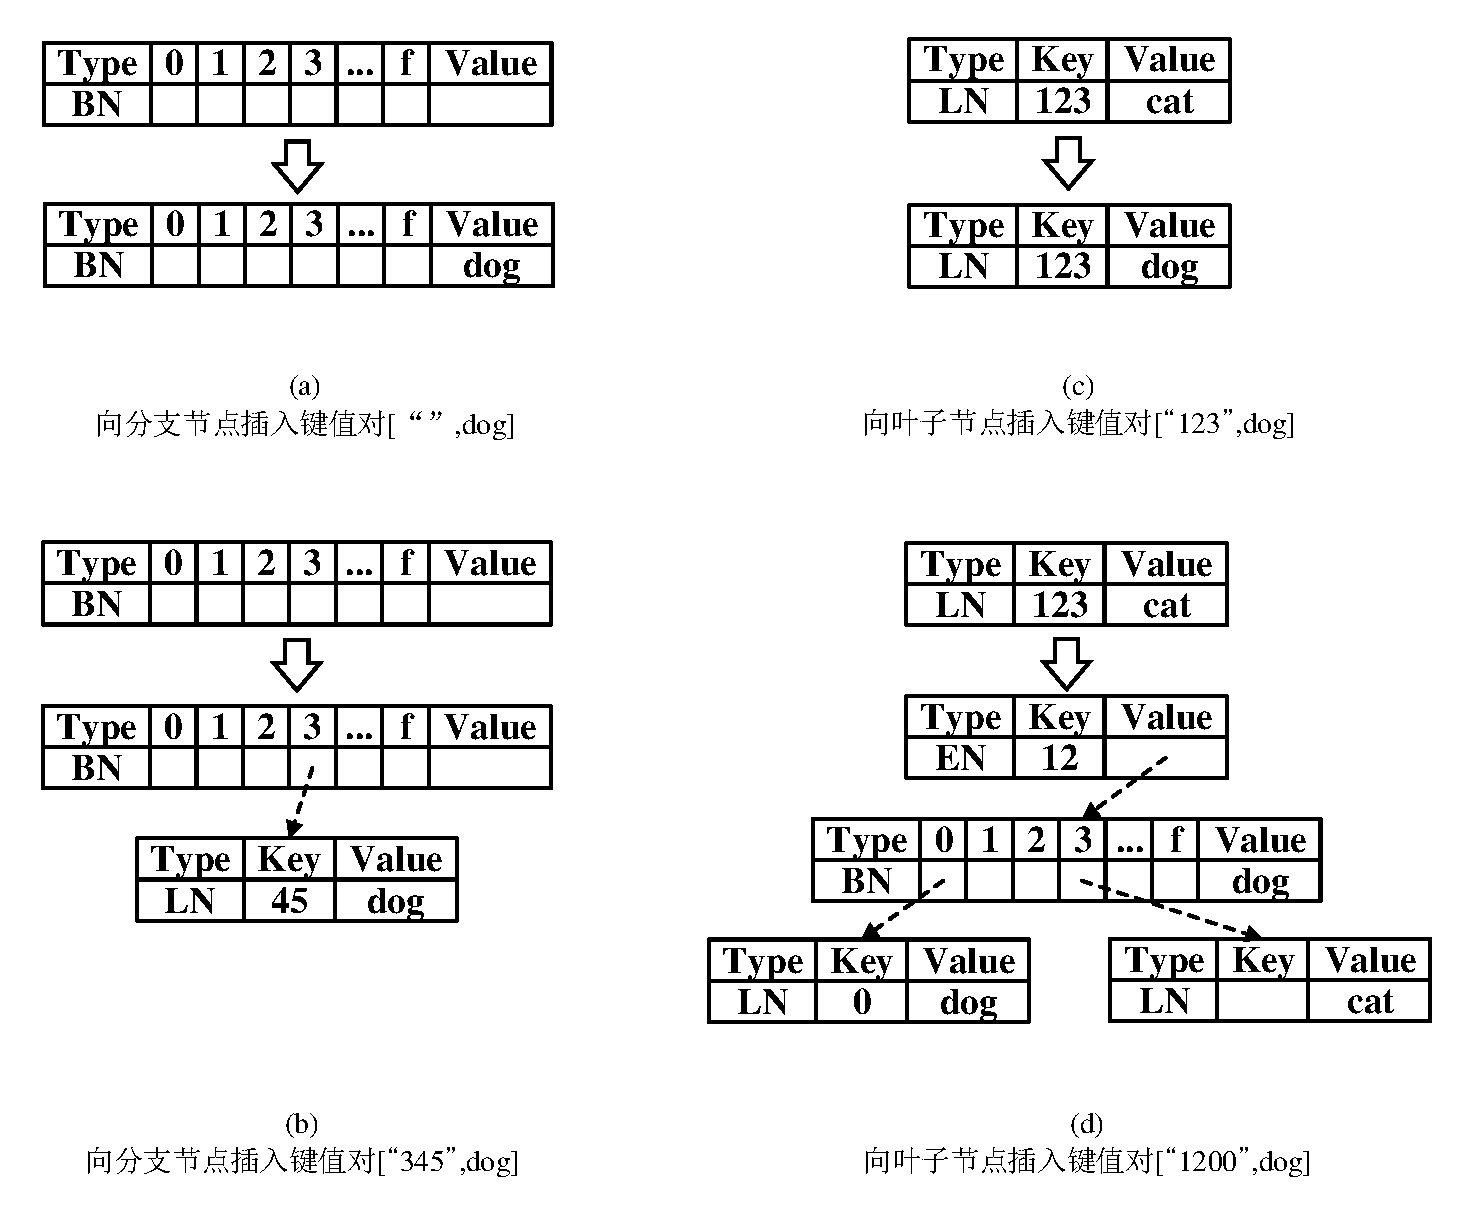
\includegraphics[width=6 in]{fig/MPTUpdate}
\DeclareGraphicsExtensions.
\caption{The Merkle Patricia Tree}
\label{fig:MPTUpdate}
\end{figure}

图~\ref{fig:MPTUpdate} 通过四个简单的例子展示了MPT树的插入过程。首先是将一个“键值对”插入到分支节点,这分为两种情况。如果当前的键空间已经为空,我们可以直接将“值”插入到分支节点的第17个位置。否则,在经过了分支节点匹配后,键空间中“剩余键”和“值”将会存储在分支节点指向的一个新的叶子节点中。其次是将“键值对”插入到叶子节点,也分为两种情况。如果当前键空间中“剩余键”与叶子节点中的“键”正好匹配,直接将叶子节点中的“值”修改为新的“值”即可。否则,我们将找到当前键空间“剩余键”和叶子节点“键”的共同前缀,将其作为一个新建的扩展节点的“键”,并新建一个分支节点,将现有的叶子节点和新建的叶子节点作为子节点插入到分支节点对应的空间中。

注意,MPT中的每一个节点都通过可递归长度前缀法~\cite{RLP_code}(Recursive Length Prefix, RLP) 进行了编码并对编码值再进行了哈希。数据库中存储了每个节点的“键值对”键值对,其中“键”为该节点RLP编码的哈希,“值”为该节点的RLP编码。这样每个节点可以通过他的哈希值被引用,同时保证了MPT的可搜索性和可验证性。通过这种方式,MPT的根哈希成为了整棵树的指纹信息,根哈希的值由所有下层节点的哈希值所决定,任何节点的微小改变都会导致根哈希的值发生变化。此外,MPT与默克尔树不同,MPT是完全确定性的,即一组相同的“键值对”采用不同的顺序插入到MPT中,最终得到的根节点哈希值是相同的,而默克尔树不具有这个性质。
%The Merkle Patricia Tree (MPT) is first proposed in Ethereum~ \cite{wood2014ethereum, merkle_patricia_tree}, which combines the Trie Tree and the Merkle Tree for data update efficiency. There are three kinds of nodes in an MPT to achieve the goal. Leaf Nodes(LN) represents [key,value] pairs. Extension Nodes(EN) represent [key,value] pairs where keys are the public prefixes and their values are the hashes of the next nodes. The Branch Nodes (BN) are used to store possible branches when the prefixes of the keywords differ, which is presented with 17 elements. Among the 17 elements, the first 16 elements represent the 16 possible hex characters in a key and the last element stores a value if a key in a [key,value] pair matches the node.

%Note that, each node of the MPT is represented by its hash and is encoded using Recursive Length Prefix (RLP) code that is mainly used to encode arbitrarily binary data~\cite{RLP_code}, which ensures the cryptographically security of the search operations. The root hash in MPT becomes a fingerprint of the entire tree and is computed based on all hashes of nodes below. Therefore, any modification in a node would incur recomputation of the root hash. Note that, the MPT is fully deterministic, meaning that an MPT with the same [key,value] pairs is exactly the same regardless of the order of insertion, which is different from the Merkle Tree.



%Searchable Encryption was first proposed by Song et al. \cite{song2000practical}, their solution allows a user to outsource its encrypted data to cloud services, and meanwhile retaining the ability to search over it. Normally, searchable encryption has been divided into two categories, i.e.,  Searchable Symmetric Encryption(SSE) and Public Key Encryption with keyword search(PKE). The most classical SSE scheme was proposed by Curtmola et al. in~\cite{curtmola2011searchable}. They defined  privacy against passive adversaries (i.e., honest but curious servers) and developed their scheme by using an inverted index. There exist various SSE schemes with different secure searching functionalities. For example, dynamic SSE schemes~\cite{kamara2012dynamic,cash2014dynamic,stefanov2014practical} allow a user to update his dataset and ranked keyword search scheme~\cite{wang2010secure} that allow a user to retrieve  ranked search results from the server. The most famous PKE scheme was proposed by Boneh et al.~\cite{boneh2004public} with the bilinear map. Normally, the efficiency of the PKE schemes are much lower than the SSE schemes.

%【SSE】Thanks for the suggestions. We explained the secure searchable encryption schemes in Section 2. Searchable encryption allows the server to perform search operations without seeing plaintext data. It empowers the server an ability to search over ciphertext and ensures the security of data on the server. In this revised manuscript, we discussed the existing categories of searchable encryption in Section 2.

\section{问题定义}
在本节中,我们将正式定义方案的攻击模型,方案需要解决的问题以及方案需要实现的目标。

\subsection{攻击模型}
在单用户场景中,数据持有者和数据搜索用户是同一人,而在多用户场景中,这两者是分开的。我们假定数据持有者本身是可信的,而数据搜索用户不可信。此外,我们假定提供存储和搜索服务的云服务器是不可信的,即 1) 云服务器会试图从用户的加密数据和搜索请求中推断出一些隐私信息; 2) 云服务器有可能会因为外部攻击、配置错误、软件错误等原因背离原有协议,从而导致产生数据新鲜性攻击和数据完整性攻击,用以节省其自身的计算开销和通信开销。数据新鲜性攻击和数据完整性攻击的正式定义如下:

\begin{definition}[\textbf{数据新鲜性攻击}]\label{def:freshness}
    {\itshape
			在对称加密搜索中,数据新鲜性攻击是指一个恶意的云服务器试图从旧数据集中返回搜索结果,而不从最新的数据集中返回搜索结果。正式地,让$\Delta_{n-1} = \{\delta_1,\delta_2,\cdots,\delta_{n-1}\}$ 代表用户数据集的历史版本, $\delta_n$ 代表用户的最新数据集,云服务器返回的搜索结果为 $\delta_i$ 的子集,其中 $1 \le i \le n-1$。
      %A data freshness attack in SSE is that a malicious server (or an attacker) attempts to return the historical version of the search result, not the most recently updated version. Formally, let $\Delta_{n-1} = \{\delta_1,\delta_2,\cdots,\delta_{n-1}\}$ denote the historical version of the dataset and $\delta_n$ is the latest version. However, the search result returned by the server is retrieved from $\delta_i$ where $1 \le i \le n-1$.
    }
\end{definition}

\begin{definition}[\textbf{数据完整性攻击}]\label{def:integrity}
    {\itshape
			在对称加密搜索中,数据完整性攻击是指一个恶意的云服务器试图篡改搜索结果,阻止数据搜索用户获取到完整的搜索结果。正式地,让 $\tau$ 代表对称加密搜索方案中的搜索令牌,$\delta_i$ 代表数据集,其中 $1 \le i \le n$。对应的搜索结果应为 $\mathcal{F}(\delta_i, \tau)$,但云服务器返回的搜索结果为 $\mathcal{G}(\delta_i, \tau)$, 其中$\mathcal{G}(\delta_i, \tau) \neq \mathcal{F}(\delta_i, \tau)$。
      %A data integrity attack in SSE is that a malicious server (or an attacker) attempts to tamper with the search result to prevent authenticated users from accessing the complete and correct search result. Formally, let $\tau$ be the search token of the SSE scheme, and $\delta_i$ be the dataset, where $1 \le i \le n$, the corresponding search result should be $\mathcal{F}(\delta_i, \tau)$, but the result returned by the server is $\mathcal{G}(\delta_i, \tau)$, where $\mathcal{G}(\delta_i, \tau) \neq \mathcal{F}(\delta_i, \tau)$.
    }
\end{definition}

%We assume that the data owner is trusted and the data users authorized by the data owner are also trusted\footnote{Please refer to Section \ref{Sec:Discussion} for details on how we can enforce such assumption in practice with multi-user access control techniques.}.
%We consider cloud services performing searchable symmetric encryption (SSE) to be untrusted, which means 1) cloud services intends to derive some sensitive information from the encrypted data and the queries; 2) cloud services may deviate from the prescribed protocols and mount a data freshness attack or a data integrity attack to save its computation or communication cost. The definitions of the data freshness attack and the data integrity attack are presented as follow:

%在可验证加密搜索中,由于服务器不诚信导致的安全性攻击主要可以分为以下两种:
%	重放攻击(Replay Attack):在加密搜索中,重放攻击是指服务器(攻击者)试图返回旧的搜索结果,而不是最新的搜索结果。我们用Δ_n={δ_1,δ_2,⋯,δ_n}来表示旧版本的数据集,用δ_(n+1)来表示最新的数据集,则服务器返回的搜索结果是数据集δ_i的搜索结果,其中1≤i≤n。
%	数据完整性攻击(Data Integrity Attack):在加密搜索中,数据完整性攻击是指服务器(攻击者)试图不让用户获取完整的搜索结果。我们用τ来表示加密搜索中用户的搜索陷门,用户应该得到的搜索结果为F(τ),而服务器返回的搜索结果为G(τ),其中G(τ)⊂F(τ)并且G(τ)可能为∅。
%重放攻击仅存在于动态的加密搜索方案中,在数据库静态的情况下不存在。但现实中,动态数据库较为常见,因此重放攻击是可验证加密搜索必须要解决的问题。数据完整性攻击不仅包括服务器少返回搜索结果的情况还包括了服务器不返回搜索结果来规避结果验证的情况。


\subsection{设计目标}

本论文旨在设计一种普适的可验证加密搜索框架,即该方案可以和任意加密搜索方案相结合,包括但不限于~\cite{stefanov2014practical,cash2014dynamic,kamara2012dynamic},使其能够完成结果验证的功能。本方案将现有的加密搜索方案当做黑盒,总体来说,需要满足以下几个需求:

\begin{enumerate}
	\item \textbf{机密性:} 数据和关键字的机密性是加密搜索最近本的安全需求。它保证了用户的明文数据和关键字信息无法被其他不可信第三方所推断。并且保证了敌手无法从方案的加密数据集,验证索引以及搜索关键字中推断出任何有用的隐私信息。
	%The confidentiality of data and keywords is the most important privacy requirements in SSE. It ensures that users' plaintext data and keywords cannot be revealed by any unauthorized parties, and an adversary cannot learn any useful information about files and keywords through the proof index and update tokens used in %\name.
	%In our scheme, data privacy and keyword privacy is guaranteed by its underlying cipher. Moreover, the search pattern of our scheme is hiding by trading the space.
	\item \textbf{可验证性:} 一个可验证的对称加密搜索方案应该能够验证搜索结果的正确性和完整性,即防止重放攻击和数据完整性攻击。%A verifiable SSE scheme should be able to verify the freshness and integrity of the search results for users.
	%In our scheme, we design a proof algorithm based on the proof structure to detect the dara integrity attacks and meanwhile use the chained-timestamp mechanism to detect the replay attacks.
	\item \textbf{高效性:} 一个可验证对称加密搜索方案应该达到次线性的计算复杂度,即对数复杂度 $O(log(|W|))$,其中 $|W|$ 是关键字的总数,并且应该在支持用户数据更新的情况下仍然能达到该复杂度。注意,这里的计算复杂度仅仅指服务器提供结果验证服务时所需的额外计算复杂度,不包括加密搜索方案本身带来的计算复杂度。%A verifiable SSE scheme should achieve sublinear computational complexity, e.g. logarithmic $O(log(|W|))$, where $|W|$ is the number of keywords, even with file update. Note that, the computational complexity only refers to the cost of searching operations for verification, which does not include the complexity of the searching operations in the existing SSE schemes.
	%Update efficiency, search efficiency and verification efficiency is the most improtant indicator we aim to achieve. In our scheme, we leverage the Mekle Patricia Tree (MPT) which provides the $O(log(n))$ efficiency for search and update which is the optimal solution to the best of our knowledge.
\end{enumerate}

	%机密性:数据和关键字机密性是加密搜索中最重要的隐私需求。其中,数据机密性要求用户的明文数据不能被云服务器获取,关键字机密性要求关键字和文件的相关性不能被云服务器所推断。
	%可验证性:一个可验证的加密搜索方案应该能够验证搜索结果的正确性和完整性,即防止重放攻击和数据完整性攻击。
	%效率:一个可验证的加密搜索方案应该在搜索和更新时具有合理的计算复杂度,例如O(log⁡(|W|)),其中|W|是关键字的数目。


  %This paper aims to provide result verification for any SSE schemes, including but not limited to~\cite{stefanov2014practical,cash2014dynamic,kamara2012dynamic}. Therefore, we treat an existing SSE scheme as a black box such that our proposed scheme can be applied to these SSE schemes for result verification.



%%% 其它部分
\backmatter

%% 本科生要这几个索引,研究生不要。选择性留下。
% 插图索引
\listoffigures
% 表格索引
\listoftables
% 公式索引
\listofequations


%% 参考文献
% 注意:至少需要引用一篇参考文献,否则下面两行可能引起编译错误。
% 如果不需要参考文献,请将下面两行删除或注释掉。
% 数字式引用
\bibliographystyle{thuthesis-numeric}
% 作者-年份式引用
% \bibliographystyle{thuthesis-author-year}
\bibliography{ref/refs}


%% 致谢
% 如果使用声明扫描页,将可选参数指定为扫描后的 PDF 文件名,例如:
% \begin{acknowledgement}[scan-statement.pdf]
\begin{acknowledgement}

  三年的研究生生涯如同白驹过隙,一晃而过。从小学到研究生,将近二十年的求学生涯即将结束,却是越长大越珍惜当学生的机会。衷心感谢导师 李琦 教授,香港城市大学 王聪 教授, 武汉大学 王骞教授对本人的精心指导。他们的言传身教将使我终生受益。

  感谢 宋奇阳 同学,以及实验室全体老师和同学们的热情帮助和支持,帮我节省了不少时间。
  本课题承蒙国家自然科学基金资助,特此致谢。

%在这三年多的科研生活里,我从各位老师和同学那儿学到了很多专业知识和研究技能。在此,我要感谢曾经给予我帮助的老师和同学。
%首先我要衷心感谢我的指导老师刘永进老师。刘老师是一个学识渊博,工作负责的老师,在这三年的科研生活中,不管是在学术指导还是在日常生活上,他都给予了我很多的关怀和帮助。他认真的工作态度和渊博的学术知识都是值得我们敬佩和学习的。
%其次,我要感谢中科院软件所的马翠霞老师。马老师是一个非常勤奋和细心的人。在每天的科研工作里,我都能感受到马老师诲人不倦,孜孜以求的态度。在我刚刚踏入科研工作的时间里,她时常指导我解决在具体工作中遇到问题的一些棘手的问题。
%然后,我要感谢中科院心理所的傅小兰老师,王甦菁博士和颜文靖博士。他们在心理学领域给予了我很多的帮助,让我顺利地完成了我的硕士毕业论文。
%最后,我要感谢与我一起工作生活的实验室伙伴们。在忙碌而充实的科研生活中,有了你们的关心和帮助,我才能在这条路上走得如此顺利。
\end{acknowledgement}


%% 附录
\begin{appendix}
\chapter{外文资料原文}
\label{cha:engorg}

\title{The title of the English paper}

\textbf{Abstract:} As one of the most widely used techniques in operations
research, \emph{ mathematical programming} is defined as a means of maximizing a
quantity known as \emph{bjective function}, subject to a set of constraints
represented by equations and inequalities. Some known subtopics of mathematical
programming are linear programming, nonlinear programming, multiobjective
programming, goal programming, dynamic programming, and multilevel
programming$^{[1]}$.

It is impossible to cover in a single chapter every concept of mathematical
programming. This chapter introduces only the basic concepts and techniques of
mathematical programming such that readers gain an understanding of them
throughout the book$^{[2,3]}$.


\section{Single-Objective Programming}
The general form of single-objective programming (SOP) is written
as follows,
\begin{equation}\tag*{(123)} % 如果附录中的公式不想让它出现在公式索引中,那就请
                             % 用 \tag*{xxxx}
\left\{\begin{array}{l}
\max \,\,f(x)\\[0.1 cm]
\mbox{subject to:} \\ [0.1 cm]
\qquad g_j(x)\le 0,\quad j=1,2,\cdots,p
\end{array}\right.
\end{equation}
which maximizes a real-valued function $f$ of
$x=(x_1,x_2,\cdots,x_n)$ subject to a set of constraints.

\newtheorem{mpdef}{Definition}[chapter]
\begin{mpdef}
In SOP, we call $x$ a decision vector, and
$x_1,x_2,\cdots,x_n$ decision variables. The function
$f$ is called the objective function. The set
\begin{equation}\tag*{(456)} % 这里同理,其它不再一一指定。
S=\left\{x\in\Re^n\bigm|g_j(x)\le 0,\,j=1,2,\cdots,p\right\}
\end{equation}
is called the feasible set. An element $x$ in $S$ is called a
feasible solution.
\end{mpdef}

\newtheorem{mpdefop}[mpdef]{Definition}
\begin{mpdefop}
A feasible solution $x^*$ is called the optimal
solution of SOP if and only if
\begin{equation}
f(x^*)\ge f(x)
\end{equation}
for any feasible solution $x$.
\end{mpdefop}

One of the outstanding contributions to mathematical programming was known as
the Kuhn-Tucker conditions\ref{eq:ktc}. In order to introduce them, let us give
some definitions. An inequality constraint $g_j(x)\le 0$ is said to be active at
a point $x^*$ if $g_j(x^*)=0$. A point $x^*$ satisfying $g_j(x^*)\le 0$ is said
to be regular if the gradient vectors $\nabla g_j(x)$ of all active constraints
are linearly independent.

Let $x^*$ be a regular point of the constraints of SOP and assume that all the
functions $f(x)$ and $g_j(x),j=1,2,\cdots,p$ are differentiable. If $x^*$ is a
local optimal solution, then there exist Lagrange multipliers
$\lambda_j,j=1,2,\cdots,p$ such that the following Kuhn-Tucker conditions hold,
\begin{equation}
\label{eq:ktc}
\left\{\begin{array}{l}
    \nabla f(x^*)-\sum\limits_{j=1}^p\lambda_j\nabla g_j(x^*)=0\\[0.3cm]
    \lambda_jg_j(x^*)=0,\quad j=1,2,\cdots,p\\[0.2cm]
    \lambda_j\ge 0,\quad j=1,2,\cdots,p.
\end{array}\right.
\end{equation}
If all the functions $f(x)$ and $g_j(x),j=1,2,\cdots,p$ are convex and
differentiable, and the point $x^*$ satisfies the Kuhn-Tucker conditions
(\ref{eq:ktc}), then it has been proved that the point $x^*$ is a global optimal
solution of SOP.

\subsection{Linear Programming}
\label{sec:lp}

If the functions $f(x),g_j(x),j=1,2,\cdots,p$ are all linear, then SOP is called
a {\em linear programming}.

The feasible set of linear is always convex. A point $x$ is called an extreme
point of convex set $S$ if $x\in S$ and $x$ cannot be expressed as a convex
combination of two points in $S$. It has been shown that the optimal solution to
linear programming corresponds to an extreme point of its feasible set provided
that the feasible set $S$ is bounded. This fact is the basis of the {\em simplex
  algorithm} which was developed by Dantzig as a very efficient method for
solving linear programming.
\begin{table}[ht]
\centering
  \centering
  \caption*{Table~1\hskip1em This is an example for manually numbered table, which
    would not appear in the list of tables}
  \label{tab:badtabular2}
  \begin{tabular}[c]{|m{1.5cm}|c|c|c|c|c|c|}\hline
    \multicolumn{2}{|c|}{Network Topology} & \# of nodes &
    \multicolumn{3}{c|}{\# of clients} & Server \\\hline
    GT-ITM & Waxman Transit-Stub & 600 &
    \multirow{2}{2em}{2\%}&
    \multirow{2}{2em}{10\%}&
    \multirow{2}{2em}{50\%}&
    \multirow{2}{1.2in}{Max. Connectivity}\\\cline{1-3}
    \multicolumn{2}{|c|}{Inet-2.1} & 6000 & & & &\\\hline
    \multirow{2}{1.5cm}{Xue} & Rui  & Ni &\multicolumn{4}{c|}{\multirow{2}*{\thuthesis}}\\\cline{2-3}
    & \multicolumn{2}{c|}{ABCDEF} &\multicolumn{4}{c|}{} \\\hline
\end{tabular}
\end{table}

Roughly speaking, the simplex algorithm examines only the extreme points of the
feasible set, rather than all feasible points. At first, the simplex algorithm
selects an extreme point as the initial point. The successive extreme point is
selected so as to improve the objective function value. The procedure is
repeated until no improvement in objective function value can be made. The last
extreme point is the optimal solution.

\subsection{Nonlinear Programming}

If at least one of the functions $f(x),g_j(x),j=1,2,\cdots,p$ is nonlinear, then
SOP is called a {\em nonlinear programming}.

A large number of classical optimization methods have been developed to treat
special-structural nonlinear programming based on the mathematical theory
concerned with analyzing the structure of problems.
\begin{figure}[h]
  \centering
  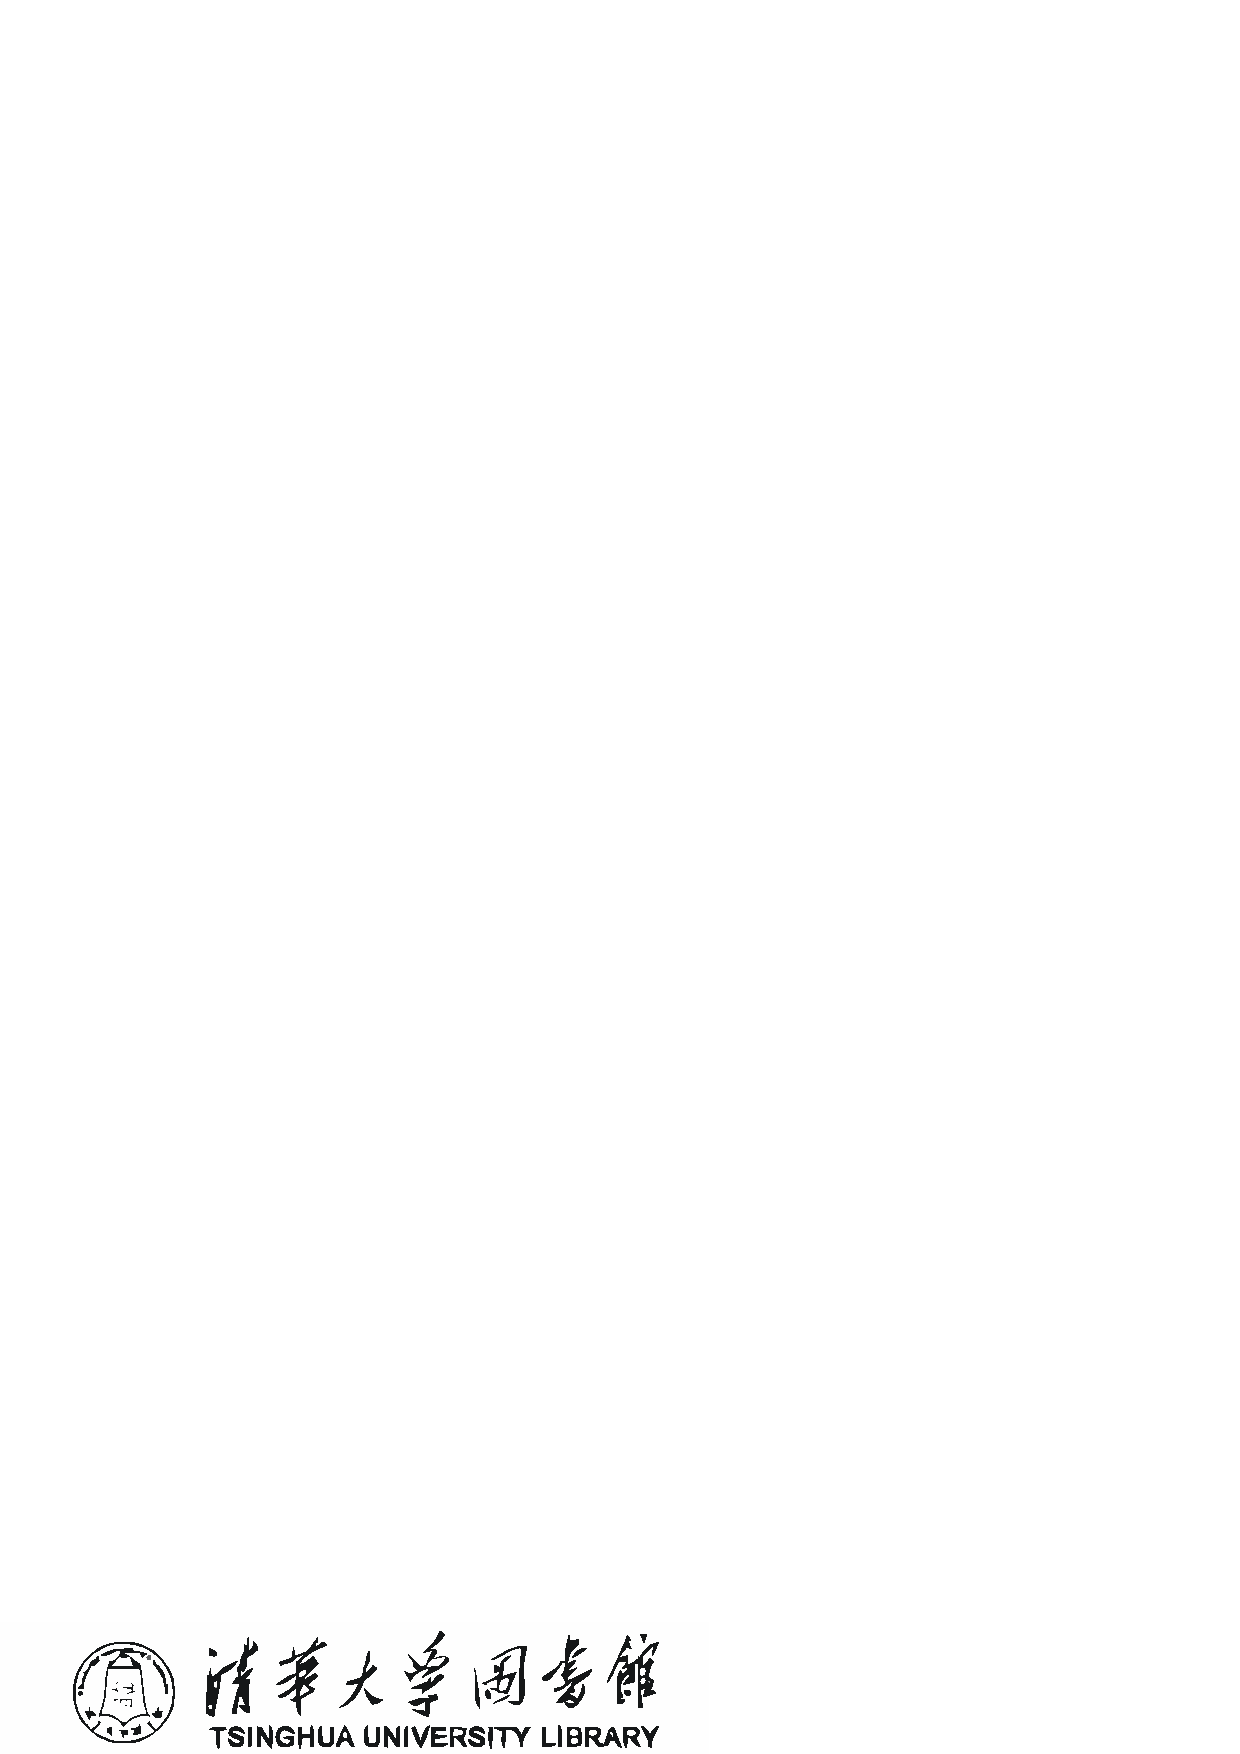
\includegraphics{thu-lib-logo}
  \caption*{Figure~1\quad This is an example for manually numbered figure,
    which would not appear in the list of figures}
  \label{tab:badfigure2}
\end{figure}

Now we consider a nonlinear programming which is confronted solely with
maximizing a real-valued function with domain $\Re^n$.  Whether derivatives are
available or not, the usual strategy is first to select a point in $\Re^n$ which
is thought to be the most likely place where the maximum exists. If there is no
information available on which to base such a selection, a point is chosen at
random. From this first point an attempt is made to construct a sequence of
points, each of which yields an improved objective function value over its
predecessor. The next point to be added to the sequence is chosen by analyzing
the behavior of the function at the previous points. This construction continues
until some termination criterion is met. Methods based upon this strategy are
called {\em ascent methods}, which can be classified as {\em direct methods},
{\em gradient methods}, and {\em Hessian methods} according to the information
about the behavior of objective function $f$. Direct methods require only that
the function can be evaluated at each point. Gradient methods require the
evaluation of first derivatives of $f$. Hessian methods require the evaluation
of second derivatives. In fact, there is no superior method for all
problems. The efficiency of a method is very much dependent upon the objective
function.

\subsection{Integer Programming}

{\em Integer programming} is a special mathematical programming in which all of
the variables are assumed to be only integer values. When there are not only
integer variables but also conventional continuous variables, we call it {\em
  mixed integer programming}. If all the variables are assumed either 0 or 1,
then the problem is termed a {\em zero-one programming}. Although integer
programming can be solved by an {\em exhaustive enumeration} theoretically, it
is impractical to solve realistically sized integer programming problems. The
most successful algorithm so far found to solve integer programming is called
the {\em branch-and-bound enumeration} developed by Balas (1965) and Dakin
(1965). The other technique to integer programming is the {\em cutting plane
  method} developed by Gomory (1959).

\hfill\textit{Uncertain Programming\/}\quad(\textsl{BaoDing Liu, 2006.2})

\section*{References}
\noindent{\itshape NOTE: These references are only for demonstration. They are
  not real citations in the original text.}

\begin{translationbib}
\item Donald E. Knuth. The \TeX book. Addison-Wesley, 1984. ISBN: 0-201-13448-9
\item Paul W. Abrahams, Karl Berry and Kathryn A. Hargreaves. \TeX\ for the
  Impatient. Addison-Wesley, 1990. ISBN: 0-201-51375-7
\item David Salomon. The advanced \TeX book.  New York : Springer, 1995. ISBN:0-387-94556-3
\end{translationbib}

\chapter{外文资料的调研阅读报告或书面翻译}

\title{英文资料的中文标题}

{\heiti 摘要:} 本章为外文资料翻译内容。如果有摘要可以直接写上来,这部分好像没有
明确的规定。

\section{单目标规划}
北冥有鱼,其名为鲲。鲲之大,不知其几千里也。化而为鸟,其名为鹏。鹏之背,不知其几
千里也。怒而飞,其翼若垂天之云。是鸟也,海运则将徙于南冥。南冥者,天池也。
\begin{equation}\tag*{(123)}
 p(y|\mathbf{x}) = \frac{p(\mathbf{x},y)}{p(\mathbf{x})}=
\frac{p(\mathbf{x}|y)p(y)}{p(\mathbf{x})}
\end{equation}

吾生也有涯,而知也无涯。以有涯随无涯,殆已!已而为知者,殆而已矣!为善无近名,为
恶无近刑,缘督以为经,可以保身,可以全生,可以养亲,可以尽年。

\subsection{线性规划}
庖丁为文惠君解牛,手之所触,肩之所倚,足之所履,膝之所倚,砉然响然,奏刀騞然,莫
不中音,合于桑林之舞,乃中经首之会。
\begin{table}[ht]
\centering
  \centering
  \caption*{表~1\hskip1em 这是手动编号但不出现在索引中的一个表格例子}
  \label{tab:badtabular3}
  \begin{tabular}[c]{|m{1.5cm}|c|c|c|c|c|c|}\hline
    \multicolumn{2}{|c|}{Network Topology} & \# of nodes &
    \multicolumn{3}{c|}{\# of clients} & Server \\\hline
    GT-ITM & Waxman Transit-Stub & 600 &
    \multirow{2}{2em}{2\%}&
    \multirow{2}{2em}{10\%}&
    \multirow{2}{2em}{50\%}&
    \multirow{2}{1.2in}{Max. Connectivity}\\\cline{1-3}
    \multicolumn{2}{|c|}{Inet-2.1} & 6000 & & & &\\\hline
    \multirow{2}{1.5cm}{Xue} & Rui  & Ni &\multicolumn{4}{c|}{\multirow{2}*{\thuthesis}}\\\cline{2-3}
    & \multicolumn{2}{c|}{ABCDEF} &\multicolumn{4}{c|}{} \\\hline
\end{tabular}
\end{table}

文惠君曰:“嘻,善哉!技盖至此乎?”庖丁释刀对曰:“臣之所好者道也,进乎技矣。始臣之
解牛之时,所见无非全牛者;三年之后,未尝见全牛也;方今之时,臣以神遇而不以目视,
官知止而神欲行。依乎天理,批大郤,导大窾,因其固然。技经肯綮之未尝,而况大坬乎!
良庖岁更刀,割也;族庖月更刀,折也;今臣之刀十九年矣,所解数千牛矣,而刀刃若新发
于硎。彼节者有间而刀刃者无厚,以无厚入有间,恢恢乎其于游刃必有余地矣。是以十九年
而刀刃若新发于硎。虽然,每至于族,吾见其难为,怵然为戒,视为止,行为迟,动刀甚微,
謋然已解,如土委地。提刀而立,为之而四顾,为之踌躇满志,善刀而藏之。”

文惠君曰:“善哉!吾闻庖丁之言,得养生焉。”


\subsection{非线性规划}
孔子与柳下季为友,柳下季之弟名曰盗跖。盗跖从卒九千人,横行天下,侵暴诸侯。穴室枢
户,驱人牛马,取人妇女。贪得忘亲,不顾父母兄弟,不祭先祖。所过之邑,大国守城,小
国入保,万民苦之。孔子谓柳下季曰:“夫为人父者,必能诏其子;为人兄者,必能教其弟。
若父不能诏其子,兄不能教其弟,则无贵父子兄弟之亲矣。今先生,世之才士也,弟为盗
跖,为天下害,而弗能教也,丘窃为先生羞之。丘请为先生往说之。”
\begin{figure}[h]
  \centering
  
\includegraphics{thu-whole-logo}
  \caption*{图~1\hskip1em 这是手动编号但不出现索引中的图片的例子}
  \label{tab:badfigure3}
\end{figure}

柳下季曰:“先生言为人父者必能诏其子,为人兄者必能教其弟,若子不听父之诏,弟不受
兄之教,虽今先生之辩,将奈之何哉?且跖之为人也,心如涌泉,意如飘风,强足以距敌,
辩足以饰非。顺其心则喜,逆其心则怒,易辱人以言。先生必无往。”

孔子不听,颜回为驭,子贡为右,往见盗跖。

\subsection{整数规划}
盗跖乃方休卒徒大山之阳,脍人肝而餔之。孔子下车而前,见谒者曰:“鲁人孔丘,闻将军
高义,敬再拜谒者。”谒者入通。盗跖闻之大怒,目如明星,发上指冠,曰:“此夫鲁国之
巧伪人孔丘非邪?为我告之:尔作言造语,妄称文、武,冠枝木之冠,带死牛之胁,多辞缪
说,不耕而食,不织而衣,摇唇鼓舌,擅生是非,以迷天下之主,使天下学士不反其本,妄
作孝弟,而侥幸于封侯富贵者也。子之罪大极重,疾走归!不然,我将以子肝益昼餔之膳。”


\chapter{其它附录}
前面两个附录主要是给本科生做例子。其它附录的内容可以放到这里,当然如果你愿意,可
以把这部分也放到独立的文件中,然后将其 \cs{input} 到主文件中。

\end{appendix}

%% 个人简历
\begin{resume}

  \resumeitem{个人简历}

  xxxx 年 xx 月 xx 日出生于 xx 省 xx 县。

  xxxx 年 9 月考入 xx 大学 xx 系 xx 专业,xxxx 年 7 月本科毕业并获得 xx 学士学位。

  xxxx 年 9 月免试进入 xx 大学 xx 系攻读 xx 学位至今。

  \researchitem{发表的学术论文} % 发表的和录用的合在一起

  % 1. 已经刊载的学术论文(本人是第一作者,或者导师为第一作者本人是第二作者)
  \begin{publications}
    \item Yang Y, Ren T L, Zhang L T, et al. Miniature microphone with silicon-
      based ferroelectric thin films. Integrated Ferroelectrics, 2003,
      52:229-235. (SCI 收录, 检索号:758FZ.)
    \item 杨轶, 张宁欣, 任天令, 等. 硅基铁电微声学器件中薄膜残余应力的研究. 中国机
      械工程, 2005, 16(14):1289-1291. (EI 收录, 检索号:0534931 2907.)
    \item 杨轶, 张宁欣, 任天令, 等. 集成铁电器件中的关键工艺研究. 仪器仪表学报,
      2003, 24(S4):192-193. (EI 源刊.)
  \end{publications}

  % 2. 尚未刊载,但已经接到正式录用函的学术论文(本人为第一作者,或者
  %    导师为第一作者本人是第二作者)。
  \begin{publications}[before=\publicationskip,after=\publicationskip]
    \item Yang Y, Ren T L, Zhu Y P, et al. PMUTs for handwriting recognition. In
      press. (已被 Integrated Ferroelectrics 录用. SCI 源刊.)
  \end{publications}

  % 3. 其他学术论文。可列出除上述两种情况以外的其他学术论文,但必须是
  %    已经刊载或者收到正式录用函的论文。
  \begin{publications}
    \item Wu X M, Yang Y, Cai J, et al. Measurements of ferroelectric MEMS
      microphones. Integrated Ferroelectrics, 2005, 69:417-429. (SCI 收录, 检索号
      :896KM)
    \item 贾泽, 杨轶, 陈兢, 等. 用于压电和电容微麦克风的体硅腐蚀相关研究. 压电与声
      光, 2006, 28(1):117-119. (EI 收录, 检索号:06129773469)
    \item 伍晓明, 杨轶, 张宁欣, 等. 基于MEMS技术的集成铁电硅微麦克风. 中国集成电路,
      2003, 53:59-61.
  \end{publications}

  \researchitem{研究成果} % 有就写,没有就删除
  \begin{achievements}
    \item 任天令, 杨轶, 朱一平, 等. 硅基铁电微声学传感器畴极化区域控制和电极连接的
      方法: 中国, CN1602118A. (中国专利公开号)
    \item Ren T L, Yang Y, Zhu Y P, et al. Piezoelectric micro acoustic sensor
      based on ferroelectric materials: USA, No.11/215, 102. (美国发明专利申请号)
  \end{achievements}

\end{resume}


%% 本科生进行格式审查是需要下面这个表格,答辩可能不需要。选择性留下。
% 综合论文训练记录表
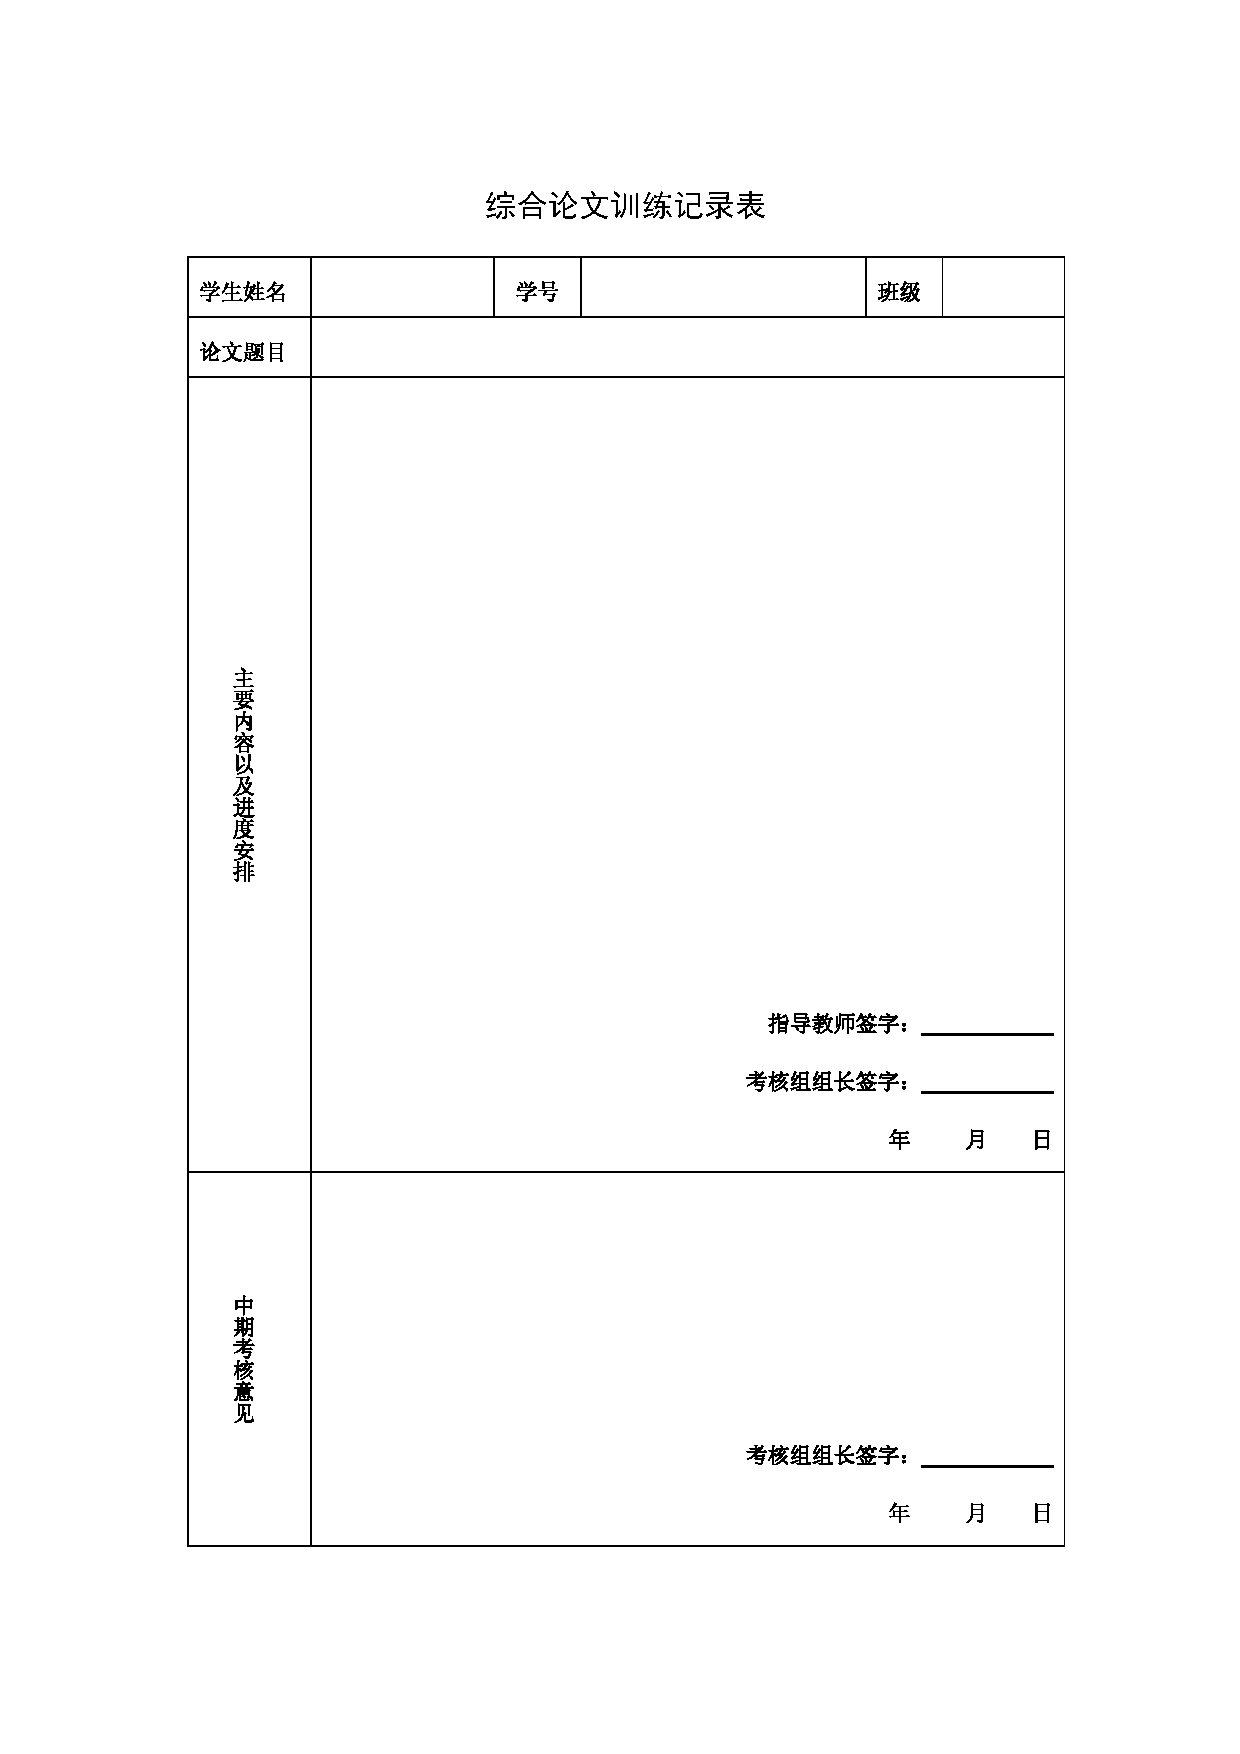
\includepdf[pages=-]{scan-record.pdf}
\end{document}
